\title{TU project proposal template}
\documentclass[12pt]{article}
\usepackage[english]{babel}
\usepackage[utf8x]{inputenc}
\usepackage{listings}
\usepackage{amsmath}
\usepackage{graphicx}
\usepackage[colorinlistoftodos]{todonotes}
\usepackage{glossaries}
\usepackage{pdfpages}
\usepackage{appendix}
\setlength{\parindent}{0em}
\usepackage{subcaption}

%%\makeglossaries
%%\newacronym{fpga}{FPGA}{Field Programmable Gate Array}
\newacronym{OSI}{OSI}{Open Standard Interface}
\newacronym{VHSIC}{VHSIC}{Very High Speed Integrated Circuit}
\newacronym{VHDL}{VHDL}{VHSIC Hardware Description Language}
\newacronym{VGA}{VGA}{Video Graphics Array}
\newacronym{bpp}{bpp}{bits per pixel}
\newacronym{TTL}{TTL}{Transistor Transistor Logic}
\newacronym{DTE}{DTE}{Data Terminal  Equipment}
\newacronym{DCE}{DCE}{Data Circuit Equipment}
\newacronym{USB}{USB}{Universal Serial  Bus}
\newacronym{UART}{UART}{Universal  Asynchronous Receiver/ Transmitter}
\newacronym{EIA}{EIA}{Electronic  Industries Alliance}
\newacronym{VDD}{VDD}{Voltage Drain Drain}
\newacronym{HSYNC}{HSYNC}{Horizontal Synchronization}
\newacronym{VSYNC}{VSYNC}{Vertical Synchronization}
\newacronym{IP}{IP}{Intellectual Property}
\newacronym{ISE}{ISE}{Integrated Synthesis Environment}
\newacronym{LSB}{LSB}{Least Significant Bit}
\newacronym{MSB}{MSB}{Most Significant Bit}
\newacronym{DAC}{DAC}{Digital to Analog Converter}
\newacronym{FIFO}{FIFO}{First In First Out}
\newacronym{LUT}{LUT}{Look Up Table}
\newacronym{ASIC}{ASIC}{Application Specific Integrated Chip}
\newacronym{IC}{IC}{Integrated Chip}
\newacronym{uart}{UART}{Universal Asynchronous Receiver and Transmitter}
\newacronym{RGB}{RGB}{Red Green Blue}
\newacronym{RAM}{RAM}{Random Access Memory}
\newacronym{XST}{XST}{Xilinx Synthesis Tool}
\newacronym{DDR SDRAM}{DDR SDRAM}{Double data rate synchronous dynamic random-access memory}
\newacronym{RTL}{RTL}{Register Transfer Language}


\begin{document}

\pagenumbering{roman}
\begin{titlepage}

\newcommand{\HRule}{\rule{\linewidth}{0.3mm}}
\center


\includegraphics[width=50mm]{tu.jpg}\\
\textsc{\LARGE \bfseries TRIBHUVAN UNIVERSITY}\\[0.5cm] % Name of your university/college
\textsc{\large \bfseries INSTITUTE OF ENGINEERING}\\
\textsc{\large \bfseries IOE CENTRAL CAMPUS, PULCHOWK}\\[0.5cm]
\textsc{Major Project Proposal} \\[0.2cm]
\Large \textbf{Title}\\[0.5cm]
%\large \textbf{Subject code} \\[0.2cm]
\bfseries
Submitted by:\\
Name (Rank)\\
Name (Rank)\\
Name (Rank)\\
Name (Rank)\\[0.5cm]

\textsc{Submitted to:}\\
\textsc{Department of Electronics and Computer Engineering}
\\[0.4cm]

{\large \today}
\vfill
\end{titlepage}

\begin{titlepage}
\center
\Large \textbf{FPGA BASED IMPLEMENTATION OF DIGITAL IMAGE PROCESSING TECHNIQUES}\\[0.5cm]
\large MINOR PROJECT REPORT\\
%\large \textbf{Subject code} \\[0.5cm]

\bfseries
Name (Rank)\\
Name (Rank)\\
Name (Rank)\\
Name (Rank)\\[0.5cm]

\textsc{SUPREVISOR}\\
\textbf{Dr ...} \\[1cm]

\textbf{"MAJOR PROJECT REPORT SUBMITTED FOR PARTIAL FULLFILLMENT OF THE DEGREE OF BACHELORS' IN ELECTRONICS AND COMMUNICATION ENGINEERING"}\\[0.5cm]
\textsc{DEPARTMENT OF ELECTRONICS AND COMPUTER ENGINEERING}\\[0.2cm]
\textbf{IOE CENTRAL CAMPUS}\\
\textbf{PULCHOWK, LALITPUR}\\[0.5cm]
\textbf{\large \today}
\end{titlepage}


\section*{Certificate of approval}
\addcontentsline{toc}{section}{Certificate of approval}
\par
The  undersigned  certify  that  they  have  read,  and  recommended  to  the  Institute  of Engineering  for acceptance of a project proposal entitled \textbf{"Implementation of Redirected Walking in Virtual Reality"} submitted by Ashu Adhikari (070/BEX/407), Bidur Wagle (070/BEX/409), Deep Shankar Pandey(070/BEX/411), Sujal Dhungana(070/BEX/442),  in partial fulfillment  of  the  requirements  for  the  Bachelor’s degree in Electronics \& Communication Engineering.  \\[2cm]
................. \\
Department of Electronics \& Computer Engineering,
\\Pulchowk Campus, Pulchowk
\\Tribhuvan University, Nepal \\[1cm]
................. \\
Department of Electronics \& Computer Engineering,
\\Pulchowk Campus, Pulchowk
\\Tribhuvan University, Nepal \\[1cm]
................. \\
\\Head of Department
\\Department of Electronics \& Computer Engineering,
\\Pulchowk Campus, Pulchowk
\\Tribhuvan University, Nepal \\[1cm]

\clearpage


\section*{Acknowledgment}
\addcontentsline{toc}{section}{Acknowledgment}

We propose to do project entitled ‘Implementation of Redirected Walking in Virtual Reality’. Our group would like to first of all express a sincere gratitude to Dr. Basanta Joshi for his immense support to build this idea and explore its feasibility. We would also like to thank Ken Ehrhart and Sujit Jha from ‘Paracosma’ for willing to share their research materials and equipment with us for the development of this project. We are also thankful to Prof. Om Prakash Gnawali from University of Houston for encouraging us to work in this project.\\
\\
The Department of Electronics and Communication surely deserves a huge thank for giving us this huge opportunity to work on this idea.\\
\\
Comments and suggestions from all the teachers and friends are highly appreciated.
\\[1cm]
Our Team
\\January 02, 2017
\clearpage
\section*{Abstract}
In this project we try to implement the redirected technique and change blindness in Virtual Reality. We will create individual virtual environments to test each of the method. We will assess the effectiveness of the method by testing the environment on human users. We will statistically analyze the extent of implementation of the techniques on the devices available to us and the virtual environment created by us. \\
\\
After conducting the studies to find the effectiveness of the techniques, we will create a singular program that will encompass all the modular experimental results, assessing the implementation capacity of the techniques.

\addcontentsline{toc}{section}{Abstract}
\clearpage

\tableofcontents
\addcontentsline{toc}{section}{Table of Contents}
\clearpage

\listoftables
\addcontentsline{toc}{section}{List of Tables}
\clearpage

\listoffigures
\addcontentsline{toc}{section}{List of Figures}
\clearpage


%%\addcontentsline{toc}{section}{List of Symbols and Acronyms}

\clearpage

\pagenumbering{arabic}
\section{Introduction}
Virtual reality (VR) typically refers to computer technologies that use software to generate realistic images, sounds and other sensations that replicate a real environment (or create an imaginary setting), and simulate a user's physical presence in this environment, by enabling the user to interact with this space and any objects depicted therein using specialized display screens or projectors and other devices. Conventional methods of navigating within a virtual reality environment involve the use of interfaces such as keyboards, hand-held input devices such as joystick, mouse and trackball and hand-worn gloves. [9] While these devices are mostly adequate, they are rather obtrusive and require some amount of training to use.\\
\\
In the real world we navigate with ease by walking, running driving, etc., but in immersive virtual environments (IVEs) realistic simulation of these locomotion techniques is difficult to achieve. Traveling through immersive virtual environments by means of real walking is an important activity to increase naturalness of virtual reality (VR) – based interactions.[16]\\
\\
One of the way to provide experience of walking is by transferring the user’s tracked head movements to changes of camera in the virtual world by means of a one-to-one mapping. Real-walking locomotion interfaces enable better user navigation, however the user must be tracked, restricting the VE size to the tracked space. [12] Thus, the large virtual worlds cannot be explored. Thus, concept for virtual locomotion methods are needed that enable walking over large distances in the virtual world while remaining within a relatively small space in the real world.\\
\\
Various prototypes of interface devices have been developed to prevent displacement in the real world. These devices include torus-shaped omni-directional treadmills, motion foot pads, motion carpets, etc.[3] One of the platform include Infinadeck omnidirectional treadmill. Although Burger's Infinadeck isn't the first omnidirectional treadmill on the markert, (the Virtuix Omni and Cyberith also aim for the same type of endless VR walking experience),  the Infinadeck sets itself apart because it uses motorized components, rather than passive, low-friction surfaces to facilitate movement.[2] Although these hardware systems represent enormous technological achievements, they are still very expensive and will not be generally accessible in the foreseeable future.\\
\\
Recently, efforts have been made to use a software solution to address the problem of simulating large spaces. [7] One of such techniques is Redirected Walking. Redirected walking is a virtual reality locomotion technique that enables users to explore a virtual world that is considerably larger than the tracked working space. With this approach the user is redirected through manipulations applied to the displayed scene, causing users to unknowingly compensate for scene motion by repositioning and/or reorienting themselves.[1] These compensations ideally permit users to explore large and potentially unbounded virtual worlds while walking naturally through a physically limited space. [6] With redirection techniques, the virtual camera is manipulated by applying gains to user motion so that virtual world moves differently than the real world.If employed using correct timing this technique can be one of the most economic and viable solution to walk users through large-scale IVEs while physically remaining in a reasonably small work space.\\
\\
Change blindness is a perceptual phenomenon that occurs when a change in a visual stimulus is introduced and the observer does not notice it. It is another of the technique being exploited to fool the users to believe them that they are in a larger virtual world while confining them to a smaller real world. By applying manipulations to the model of the virtual world, it can be demonstrated that a user can seamlessly walk through a virtual environment that is an order of magnitude larger than the physical work space. In contrast to previous redirection techniques, this approach, based on a dynamic, adaptive environment model, does not introduce any visual vestibular conflicts from manipulating the mapping between physical and virtual motions, nor does it require breaking presence to stop and explicitly reorient the user. [20] However, it does impose a different set of constraints with regards to environment geometry and user motion.\\
\\
In this project we want to test the limits to which the devices available to us can implement redirected walking. Then, using those techniques we will try to create a simple game in Virtual Reality, encompassing these methods.




\clearpage
\section{Previous Works}
In a 2001, Razzaque et al [13] observed the first successful implementation of redirected walking. In their study, the user was directed to press a series of buttons inside the virtual world in a simulated fire drill. User were directed to press these buttons which were in a zig-zag pattern in virtual world. Each time the user turned in the virtual environment, a negative rotational gain was applied causing the user to physically turn 180 degrees in the real world for a turn of angle slightly over 90 degrees in the virtual world. This caused the users to walk back and forth in the real world while following a zig-zag pattern in the virtual world.\\
\\
In 2004, Kuhl [10] conducted a virtual reality study in which subjects' rate of rotation was manipulated. Subjects were not told about the rotational gain, but they were given tasks to acclimate them to the difference compared with their real-world rotation. After this practice, the subjects were asked to perform accurate rotations without the benefit of visual feedback. The result of the study indicated that, given a small amount of practice, users are able to adjust their expectations to accurately measure their rotation even without visual feedback when a rotational gain is applied. This result suggested that the rotational gain technique applied by Razzaque et al might be generalizable.[22]\\
\\
In 2008, Steinicke et al [16] set about quantifying the perceptual thresholds at which users can detect various visual manipulations in virtual environments.
The following list summarizes specific numerical outcomes. Subjects did not detect:
	
\begin{itemize}
\item rotational gains below +68\%;
\item	rotational gains above -10\%;
\item	translational gains within +/-22\%;
\item	curvature gains along a circle with a radius of at least 24m.

\end{itemize}
\clearpage
\section{Objective}
\begin{itemize}
\item To create a virtual environment to experiment on redirection techniques and leveraging change blindness.
\item Explore and Compare the limits of redirection techniques and change blindness.
\item If possible, implementation of those techniques to create a simple game.
\end{itemize}

\clearpage

\section{Methodology}
Enumerating the tasks involved in the project, would most probably illuminate the project and how it works. The project can be broken down into following simpler phases:
\begin{enumerate}
\item Making of Virtual Environment 
\\
It is an iterative process. We need to create different types of environment for each of the technique being applied. 
\begin{itemize}
\item Import assets from Unity Library
\item Search assets from Online Open Source Library
\item Modify the properties and script the assets using C\#
\end{itemize}
\item Implementation of Technique
\\
The techniques include translational gain, rotational gain and curvature gain in redirected walking technique and change blindness. The following tasks will be incorporated for each of the techniques.
\begin{itemize}
\item Use SteamVR API to get the information on location and movement of user
\item Bring out changes in the transformation matrix to implement the redirected walking
\item Change the map of virtual environment depended upon the orientation of user
\end{itemize}
\item Finding limits and patterns
\begin{itemize}
\item Explore the above scenes with human users
\item Take reviews and suggestion from the users to find the effectiveness of the method
\item Perform statistical analysis on effectiveness of the technique with changes in their respective parameters.
\end{itemize}
\item If possible finalize the implementation to create a simple game in VR.
\end{enumerate}
\clearpage
\subsection{System Block Diagram}
The generalized system block diagram of the proposed system can be viewed as below:
\begin{figure}[!ht]
\centering
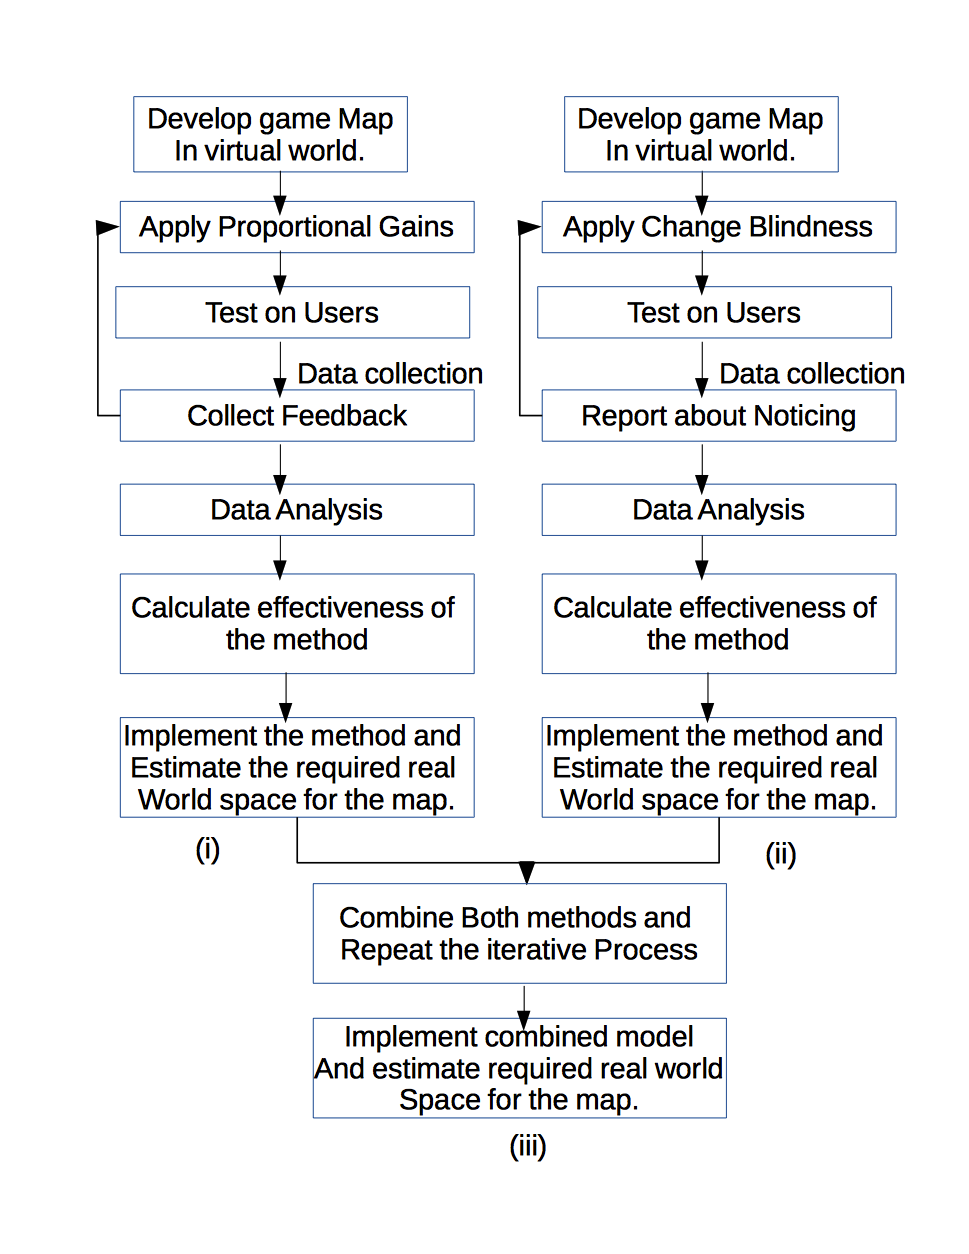
\includegraphics[width = 0.9 \textwidth]{SBD_Redricted_walking}
\caption{System Block Diagram}
\end{figure}
\clearpage
\subsection{Flowchart}
The system is expected to follow following work flow:
\begin{figure}[!ht]
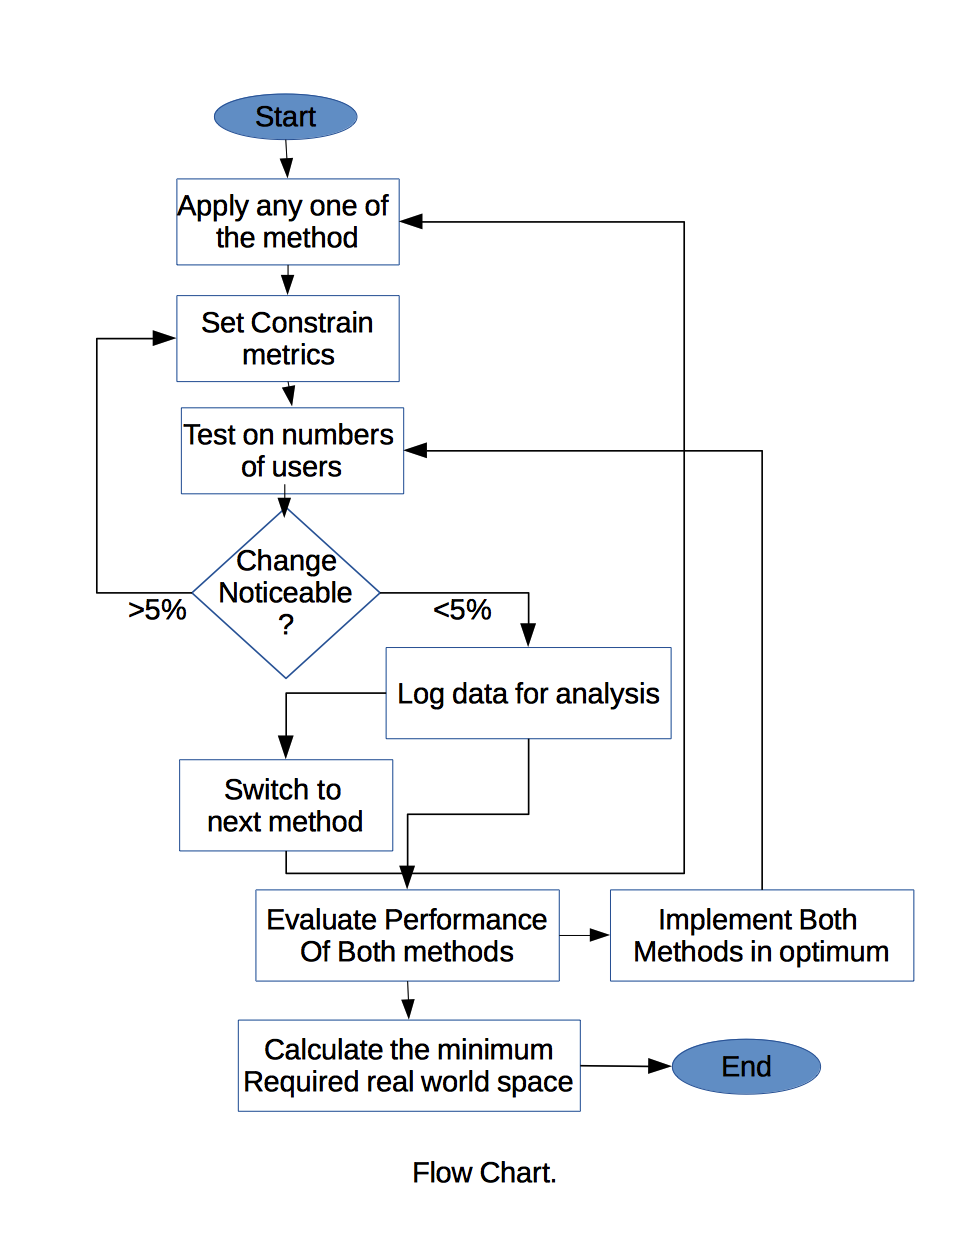
\includegraphics[width = 0.8 \textwidth]{FlowChart}
\caption{Flow Chart}
\end{figure}

\clearpage
\subsection{General Technique and Algorithm}
Redirected walking can be applied via gains which define how tracked real-world movements are mapped to the virtual environment. These gains are specified with respect to a coordinate system. For example, gains can be applied by uniform or non-uniform scaling factors applied to the scene coordinate system. Previous research approaches suggest defining locomotion gains with respect to the user’s walking direction [8].\\
\\
We use the user’s locomotion triple (s,u,w) defined by three vectors: the strafe vector s, the up vector u and the direction of walk vector w. The user’s direction of walk can be determined by the actual walking direction.The strafe vector is orthogonal to the direction of walk and parallel to the walking plane. While walking the user’s up vector is usually given by the inverse of the gravitation direction, which is the main concern with our experiment.
\subsubsection{Translational Gain}
We need to first calibrate and register the tracking and virtual world coordinate systems. Tracking system detects and updates the vector \textit{translation}, which is updated as \textit{translation} $= current\_position - previous\_position$. Then, the \textit{translation} is applied to the virtual camera. The translational gain $g_{trans}$ $\epsilon$ R is defined by the quotient of the applied virtual world translation \textit{translation}$_{virtual}$ and the tracked real world translation \textit{translation}$_{real}$, i.e.,
$g_{trans} = \frac{translation_{virtual}}{translation_{real}}$\\
\\
When a translation gain $g_{trans}$ is applied to a translational movement \textit{translation}$_{real}$, the virtual camera is moved by the vector $g_{trans}$.\textit{translation}$_{real}$ in the corresponding direction.Translation gains are defined with respect to the user’s locomotion triple. The exploration of large ground in a small room will expect a $g_{trans}$ $\approx$ 10. Similarly, if the VR game expects to create miniature models of toys and limit the area to say a table then the $g_{trans}$ $\approx$ 0.2 is suitable.\\
\\
Besides scaling movements in the direction of walk, lateral and vertical movements are affected by uniform gains. Sometimes, uniform gains are often inadequate. Non-uniform translation gains are used to distinguish between movements in the main walking direction, lateral movements and vertical movements.\\
\\
The effectiveness of the translational gain can depend upon varieties of factor. One of the factors can be speed of the user as mentioned in the study of Neth et al. [11] We are hoping to explore the effectiveness of translational gain with respect to stride length of the user.
\subsubsection{Rotational Gain}
A real-world head turn can be specified by a vector consisting of three angles, i.e., yaw, pitch and roll. The tracked orientation change is applied to the virtual camera.Analog to translation gains, a rotation gain $g_{rot}$ is defined by the quotient of the considered component (yaw/pitch/roll) of a virtual world rotation \textit{rotation}$_{virtual}$ and the real world rotation \textit{rotation}$_{real}$, i.e.,
$g_{rot} = \frac{rotation_{virtual}}{rotation_{real}}$\\
\\
When a rotation gain $g_{rot}$ is applied to a real world rotation the virtual camera is rotated by $g_{rot}$.\textit{rotation}$_{real}$ instead of \textit{rotation}$_{real}$. This means that if $g_{rot}$ = 1 the virtual scene remains stable considering the head’s orientation change. For $g_{rot}$ $>$ 1 the virtual scene appears to rotate against the direction of the head turn, and$g_{rot}$ $<$ 1 causes the scene to rotate in the direction of the head turn. Gains are defined for each component of the rotation, i.e., yaw, pitch, and roll, and are applied to the axes of the locomotion triple.
\subsubsection{Curvature Gain}
The curvature gain $g_{cur}$ denotes the bending of a real path. For example, when the user moves straight ahead a curvature gain that causes reasonably small iterative camera rotations to one side forces the user to walk along a curve in the opposite direction in order to stay on a straight path in the virtual world. The curve is determined by a circular arc with radius r, where $g_{cur}$ $= \frac{1}{r}$. [5] The resulting curve is considered for a reference distance of r meters. In the case that no curvature is applied r = $\infty $ and $g_{cur}$ = 0, whereas if the curvature causes the user to rotate by 90 clockwise after r meters the user has covered a quarter circle and $g_{cur}$ = 1. Alternatively, a curvature gain can be applied as translation offset while the user turns the head and no translational movements are intended.
\begin{figure}[!ht]
\centering
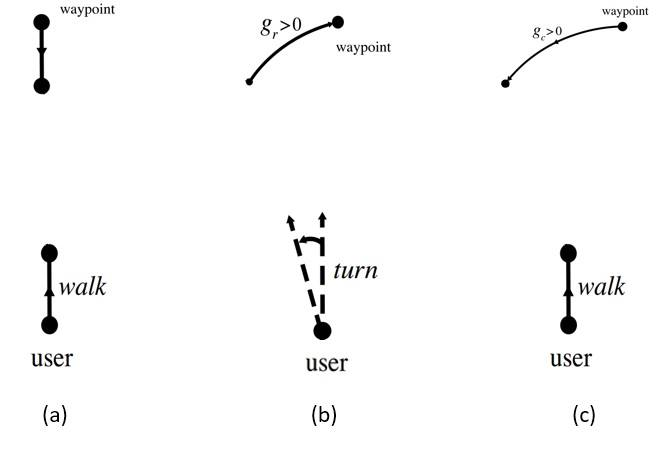
\includegraphics[width = 0.7 \textwidth]{Techs}
\caption{Graphical Illustration of three techniques}
\end{figure} \\
\begin{figure}[!ht]
\begin{subfigure}{0.5\textwidth}
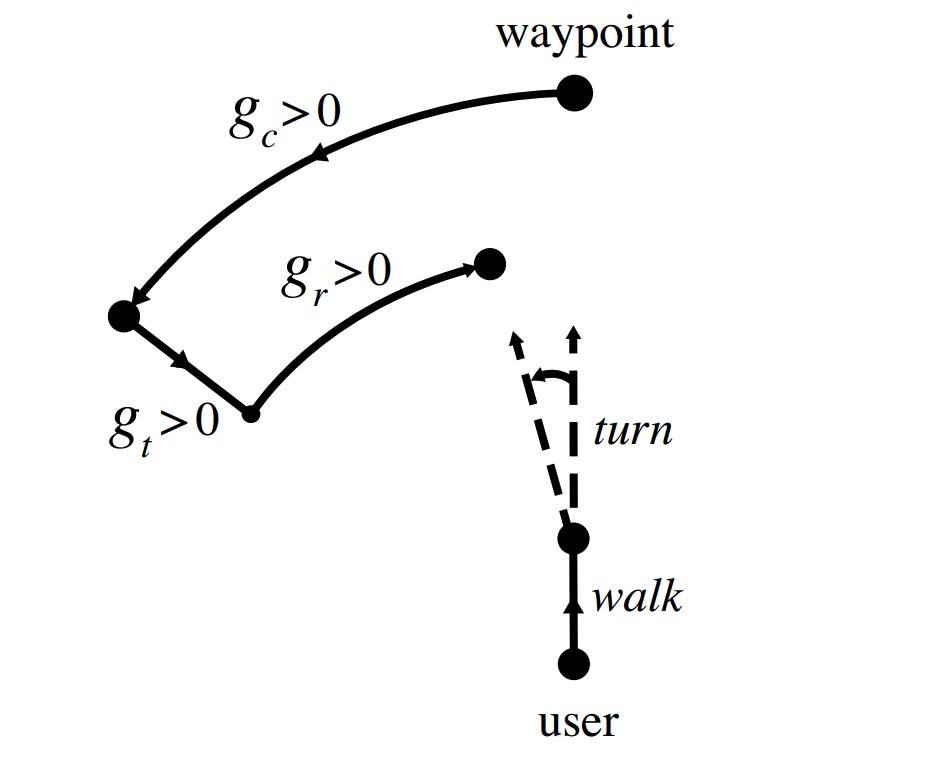
\includegraphics[width=0.9\linewidth, height=5cm]{comb} 
\caption{Combined effect of three techniques }
\label{(a)}
\end{subfigure}
\begin{subfigure}{0.5\textwidth}
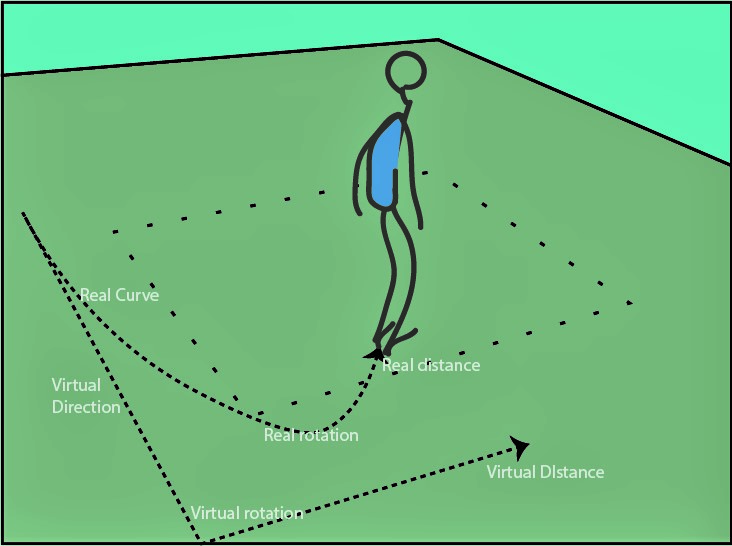
\includegraphics[width=0.9\linewidth, height=5cm]{translation2}
\caption{Implementation of combined technique in real application}
\label{(b)}
\end{subfigure}
\caption{Combination of Techniques}
\end{figure}
\clearpage



\subsubsection{Change Blindness Technique}
%% Write about this sub section here.
This technique involves manipulation of the virtual environment behind the user's field of view. User do not notice the slight changes in environment which they are not acquainted with and these variations can be used to limit the area of real world required in order to map the virtual world. This method is practically more useful in indoor scenarios like exploring a building with number of rooms, where the user enters into one room through a door and explores the room, while the user explores the room the door is rotated through 90 degrees so that the user can be redirected into another different direction. The change blindness technique can also be applied to scene geometry with certain limitations such that the user would not notcie the changes. 

\begin{figure}[!ht]
\centering
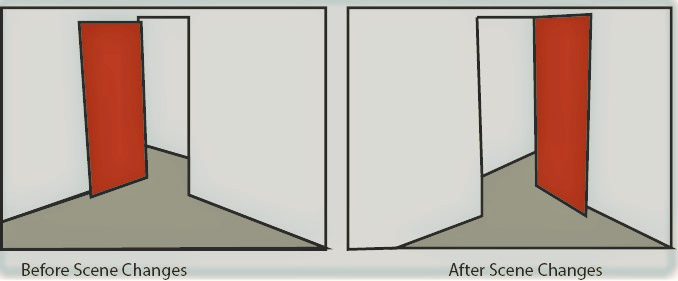
\includegraphics[width = \textwidth]{blindness2}
\caption{A simple implementation of change Blindness}
\end{figure}

\clearpage
\subsection{Tools Used}

\subsubsection{HTC Vive}
 HTC Vive is a virtual reality headset developed by HTC and Valve Corporation. This headset is designed to utilize "room scale" technology to turn a room into 3D space via sensors, with the virtual world allowing the user to navigate naturally, with the ability to walk around and use motion tracked hand held controllers to vividly manipulate objects, interact with precision, communicate and experience immersive environments.[4] It comes with 2 IR based base stations to track the user and controller in room-scale and give user the real sensation of walk in virtual world. Each base station has 120 degree field of view and can track the user and controller with high precision within a range of 5m between the base stations diagonally. The precision can be traded for larger play area.
\subsubsection{Unity 3D}
Unity is a cross-platform game engine which is basically used to develop games for PC, mobile devices and websites. It supports altogether of 21 platforms and has a great emphasis on portability, i.e uses Direct3D for Windows, OpenGL for Mac and OpenGL ES for mobile devices. 
It has a relatively simple interface for designing and allows scripts to be written both in csharp and UnityScript(javascript for unity). It is a cross platform game engine and it is both 2D and 3D oriented. It is one of the most popular game development platforms and one of the primary reasons is because of its greatly simplified game development workflow.
Not only that, but Unity has one of the best supports for the VR/AR development. Unity has built in suport for many of the VR devices such as oculus and HTC Vive, which greatly simplifies the VR projects. It gets very easy for implementing things like leap motions and sensing inputs from VR devices in virtual environment making unity3d one of the ideal choices for implementing redirected walking in VR. 
\subsubsection{SteamVR SDK \& OpenVR API}
The SteamVR SDK allows developers to target a single interface that will work with all major virtual reality headsets from seated to room scale experiences. Additionally, it provides access to tracked controllers, chaperoning, render models for tracked devices, and includes examples for using Unity's various UI systems in VR. SteamVR's compositor allows you to preview your content in VR using Unity's play mode, while leaving the normal game window to act as your companion screen on the main monitor.
\\ The OpenVR API provides a game with a way to interact with Virtual Reality displays without relying on a specific hardware vendor's SDK. It can be updated independently of the game to add support for new hardware or software updates. The API is implemented as a set of C++ interface classes full of pure virtual functions. When an application initializes the system it will return the interface that matches the header in the SDK used by that application. OpenVR API causes the game to connect to any attached VR hardware.
\\ 


\clearpage

\section{Expected Results}
\begin{itemize}
\item Development of different virtual environments necessary for implementation of different techniques.
\item Testing the environments with number of users and approximate the range of changes without being noticed significantly by the user.
\item Calculating the extend of both methods and find out which one suits for specific purposes.
\item Implementing both the methods first individually and record the decrements in required space and then combining the both technique and comparing the decrements with previous outcome.
\item Development of  some rules or patterns to follow in order to confine a virtual map within limited real world space.
\item Implementation of the results to develop a game with sufficiently large virtual environment mapped into relatively small real world space.
\end{itemize}

\clearpage
\section{Scopes}
Every major tech  companies are thriving to produce virtual reality products and it's clear that VR has become the next big thing in tech world. In one way or another VR is going to be major concern over few years. Virtual reality first came up with gaming and has grown out of limits, from Gaming to space exploration, from medicine to jet engines VR is taking it's places in various fields and has provided lots of advantages in respective areas. Walking is the most basic and intuitive way of mov- ing within the real world. Taking advantage of such an active and dynamic ability to navigate through large immersive virtual environments (IVEs) is of great interest for many 3D applications demanding loco- motion, such as urban planning, tourism, 3D games etc. [15] Three-dimensional virtual environments (VEs; virtual reality worlds) are capable of providing rich visual information, but there is strong evidence that visual information on its own is not sufficient if we are to navigate VEs as efficiently as we navigate in the real world.[14] Still one of the limitation of VR has been the limitation of real world space such that it can map and at the same time give the real sensation of walk in infinite virtual environment with the user walking naturally within a specified area. This limitation has been attempted to be fulfilled partially by means of technique like Redirected walking and change blindness but significant achievements and practical implementation is still on rudimentary stages.\\
\\The results from these methods can be implemented in larger scale in any kind of game maps or even the virtual tours of any place. The data and analytic  obtained will show the practical limitations and the implementation phase will give the effectiveness of the techniques in real example.These techniques will multiply the area of the virtual world making it possible to be explored from a small room. 
\clearpage
\section{Cost Estimation}
\begin{table}[!ht]
\centering
\begin{tabular} { |l | l | l |}
\hline
SN & Particular & Cost \\ \hline
1  & HTC Vive*    &  \$800 \\ \hline
2 & HMD BackPack Laptop*  & \$2000 \\ \hline
3 & Software Development & \$200 \\ \hline
4 & Developing Test environment & \$100 \\ \hline
5 &  Test subjects  & \$5 (per person) \\ \hline
6 & Human Resources & \$200 (per person) \\ \hline
 & \textbf{Total*} & \$ \textbf{1500}\\ \hline
\end{tabular}
\caption{Cost Estimation of the Project}
\end{table}
\small * The particulars would be borrowed for development and presentation purposes. 

\clearpage
\section{Time Schedule}
\begin{table}[!ht]
\centering
\begin{tabular} { |l | l | l |}
\hline
SN & Activity & Time \\ \hline
1 & Getting acquainted with Unity 3D     &  1 week \\ \hline
2 & Getting acquainted with HTC Vive controls & 1 week \\ \hline
3 & Import relevant assets from Unity 3D and modify their properties using C\# &  2 weeks \\ \hline
4 & Search relevant assets on the internet and modify their properties & 1 week \\ \hline
5 & Create required Graphical images in Blender & 2 weeks \\ \hline
6 & Assemble above assets to create a virtual environment & 2 weeks \\ \hline
7 & Create virtual environment for checking translational gain effects & 2 weeks \\ \hline
8 & Test and observe the above environment on human user& 1 week \\ \hline
9 & Create virtual environment for checking rotational gain affects & 2 weeks \\ \hline
10 & Test the above environment on human user& 1 week \\ \hline
11 & Create virtual environment for checking curvature gain affects & 2 weeks \\ \hline
12 & Test the above environment on human user& 1 week \\ \hline
13& Create virtual environment for checking effectiveness of change blindness  & 1 week \\ \hline
14 & Test the above environment on human user& 1 week \\ \hline
15 & Perform statistical analysis on findings of techniques & 2 weeks \\ \hline
16 & Create a simple game based on above techniques & 4 weeks \\ \hline
17 & Testing,Debugging and Performance analysis & 1 week \\ \hline
18 & Finalization and Documentation & 2 weeks \\ \hline
\end{tabular}
\caption{Time Estimation for the Work Flow}
\end{table}

\clearpage





\appendix
\section*{Appendix}
\addcontentsline{toc}{section}{Appendix}
\subsection*{Razzaq's Experiment}
\begin{figure}[!ht]
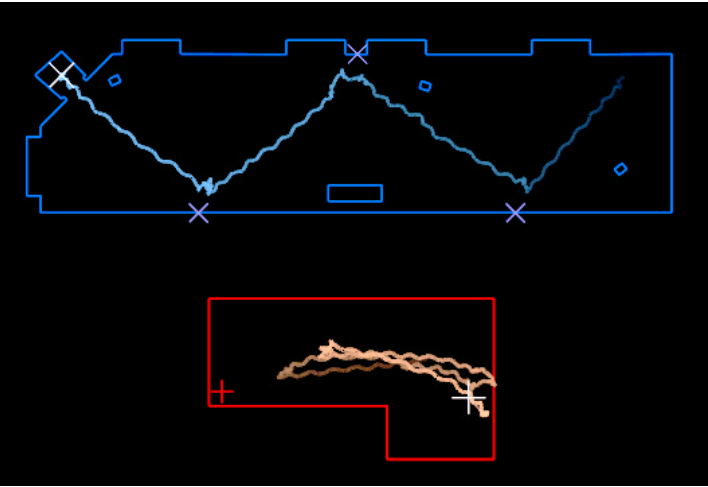
\includegraphics[width = 0.5 \textwidth]{Razzaq}
\caption[Razzaq's Experiment]{Overhead views of the path taken by the user in the virtual environment (above in blue) and the laboratory (below in red).}
\end{figure}
\subsection*{Change Blindness Experiment}
\begin{figure}[!ht]
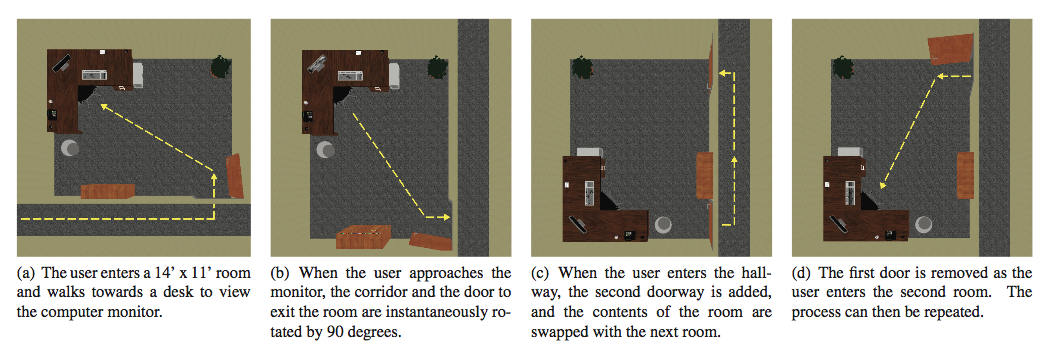
\includegraphics[width = 0.8 \textwidth]{Change_Blindness}
\caption[Change Blindness Experiment]{A step-by-step explanation of our proof-of-concept implementation of change blindness redirection. Dynamic modifications to the virtual environment model prevent users from walking outside the boundaries of the 14’ x 14’ work space as they transition between two rooms in the virtual world.}
\end{figure}



\clearpage
\nocite{*}


\clearpage
\bibliographystyle{plain}
\bibliography{source}
\addcontentsline{toc}{section}{References}

\end{document}
